\section{缓存设计}

\cpuname 中,设计实现了指令Cache和数据Cache,且均为虚拟索引物理标签(VIPT)记录,二者的突发传输数量、大小、组相联数量均为可配置。其中数据Cache支持写缓冲,以减少写回的阻塞数量。

\subsection{内存管理}
MIPS指令系统对操作模式和存储访问类型进行了严格的限定,将整个4 GB大小的虚地址空间划分为5段,如图\ref{img:mmu}所示。

虚拟地址到物理地址的翻译上,共有两种方式:一是直接地址翻译,对应图中Unmapped段,翻译较快,延迟较少;二是映射地址翻译,对应图中Mapped段,需要访问TLB表项,延迟较大。在\cpuname 的缓存设计中,通过多级TLB的方式,减少映射地址翻译模式的时延和缺失率,以在实际地址翻译中,可以综合使用直接地址翻译和映射地址翻译。

缓存使用上,指令Cache和数据Cache均支持Uncached段的单独处理,这样发送AXI请求时,只需要做指令和数据请求的两路仲裁即可,极大简化仲裁逻辑。

\begin{figure}[htpb]
    \centering
    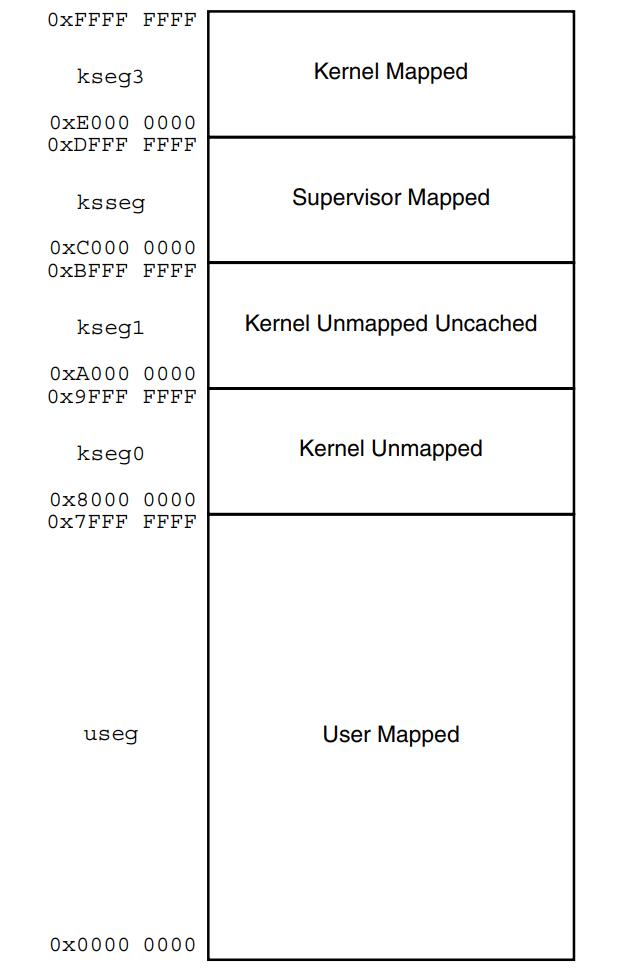
\includegraphics[width=0.3\linewidth]{mmu.png}
    \caption{虚实地址映射关系图}
    \label{img:mmu}
\end{figure}

\subsection{缓存结构}
\cpuname 的缓存结构和资源使用如图\ref{img:struct}所示,指令Cache默认为二路组相联且一路4KB,一行data共2字64bit,一行tag对应8行data;数据Cache默认为二路组相联且一路4KB、一行data共1字32bit,一行tag对应16行data。因为Bram读取数据时需要一周期后返回数据,故我们提前发送了下一个访存地址(指令Cache对应pc\_next,数据Cache对应E阶段的访存地址)进行提前查询。当到达对应的访存阶段时(指令Cache对应F阶段,数据Cache对应M阶段),在根据上一周期的命中情况判断能否同周期获取对应数据,以及是否发送AXI请求。在具体访问AXI时,Cached请求支持突发传输,默认为16字突发(即一个tag对应的总字数);Uncached请求默认不支持突发传输。

\begin{figure}[htpb]
    \centering
    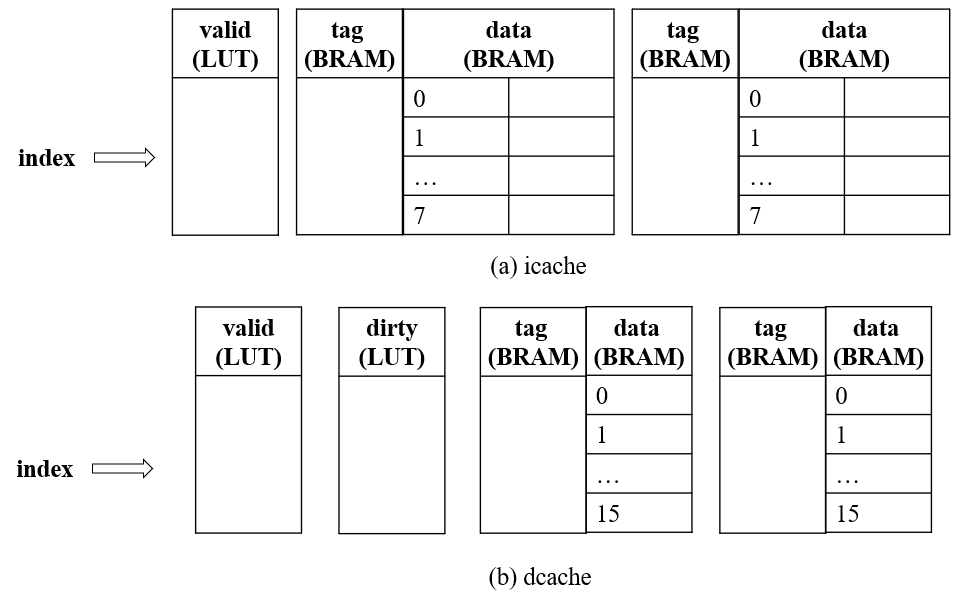
\includegraphics[width=0.6\linewidth]{cache_struct.png}
    \caption{\cpuname 缓存结构示意图}
    \label{img:struct}
\end{figure}

\subsection{CACHE指令}
在MIPS指令系统中,CACHE指令要求清除特定地址或索引位置的数据缓存。由于清除“索引位置”已经包含了清除“特定地址”,故\cpuname 的设计中,Data Cache操作全部实现为Index Writeback Invalid,Instruction Cache操作全部实现为Index Invalid,这使我们能够在满足运行操作系统所必备执行修改后的指令以及刷新DMA缓冲区的情况下,简化Cache的逻辑,使CPU能够实现更高的频率。

\subsection{状态机}
Cache的控制实现上,我们采用状态机控制的方式,状态转换的情况如图\ref{img:cache}所示,其中,Data Cache包含写回操作,故比Inst Cache多一个“CACHE\_WRITEBACK”状态,即图中绿色部分。

各个状态的含义如下。
\begin{itemize}
    \item \textbf{IDLE}:Cache空闲状态,进行数据提前读取、地址L1TLB查询或直接翻译。
    \item \textbf{TLB REFILL}:L1TLB缺失时,查找L2TLB、处理可能遇到的TLB重填异常或TLB无效异常、L2TLB命中后更新L1TLB。
    \item \textbf{UNCACHE}:向AXI发送读请求或写请求(无突发传输),并等待AXI访存结束。
    \item \textbf{CACHE REPLACE}:cache缺失后,若没有脏位,需要重新向AXI发送读请求(突发传输),访存并替换对应路的缓存行。其中替换原则采用1bit替换方式。
    \item \textbf{CACHE WRITEBACK}:当需要清除或替换缓存行时,若存在脏位,则需要将脏数据写回,即向AXI发送写请求(突发传输)。
    \item \textbf{SAVE RESULT}:当Cache因为TLB缺失或Uncached导致Cache暂时无法正常访问数据时的保留状态。
\end{itemize}

\begin{figure}[htpb]
    \centering
    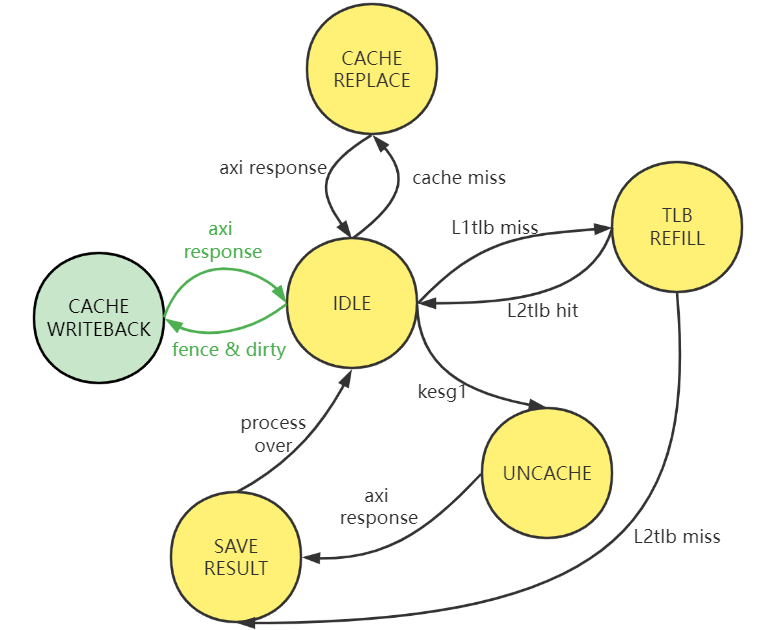
\includegraphics[width=0.8\linewidth]{cache.png}
    \caption{\cpuname 缓存状态机示意图}
    \label{img:cache}
\end{figure}

\subsection{写缓存}
在\cpuname 的设计中,对于Uncached的AXI写请求,我们设置了Store Buffer,即一个写请求队列,将AXI写请求数据缓存下来,再逐个写回,该期间如果没有Cached的访问AXI请求,则流水线不会因为写回Store Buffer数据而阻塞,提高了流水线的执行效率。

值得注意的是,为了保证读写数据的准确,当Cached数据需要访问AXI时,若这个时候Store Buffer仍然在占用AXI通道,则需要等待Store Buffer写完后,高速缓存才能去处理这个Cached数据请求,这个阶段流水线会因为该Cached数据请求得不到响应而阻塞。